\documentclass[thesis.tex]{subfile}
\begin{document}
\chapter{Distributed State Estimation} \label{Distributed State Estimation}
This section describes the distributed state estimation system created with the robot\_localization package \cite{MooreStouch2014}, \cite{Moore}. The overarching concept behind this system is for individual robots to use their sensor data to create pose estimates for the other robots in their environment. The pose estimates are then sent to the other robots and integrated into their own personal pose estimate, allowing for more accurate localization.
  
\section{Theory} \label{Theory}
\glspl{kf} perform better with more inputs. This is the driving force behind increasing the accuracy of mobile robot localization. With more sensor inputs, noise can be removed more accurately. One way to increase the number of sensor inputs to a filter is to add more sensors to the robot. However this will rapidly drive up cost and complexity. Another solution is to have robots share their information about the surrounding world, thus artificially inflating the number of sensors a robot has.

The flow for this system is as follows. A robot at position $p_l$, where $l$ represent that this position is with respect to the local frame, detects another robot at position $g_l$. The robot at $p_l$ then calculates its' pose in with respect to the global frame, $p_g$ and then transforms $g_l \rightarrow g_g$. This position $g_g$ is then shared with the robot's in the surrounding environment, which integrate the position into their own localization estimate. This is summarized below.
\begin{align}
\text{\gls{kf} output} &\rightarrow p_l, p_g \\
\text{Lidar scan} + p_l &\rightarrow g_l \\
g_l &\rightarrow g_g \\
g_g &\rightarrow \text{\gls{kf} input}
\end{align}

\section{Methods}
The following sections describes how the position estimates $p_l$, $p_g$, $g_l$, and $g_g$ are obtained.

\subsection{Coordinate Systems}
First, it is necessary to understand the naming terminology for the coordinate systems used in this discussion. The system used is identical to the \gls{ros} standard, REP-105 \cite{REP_105}. There are three different coordinate frames: $map$, $odom$, and $base_link$.

\subsubsection{Base\_Link Frame}
The base\_link frame is the simplest to understand. It is a rigidly fixed frame attached to the base of the mobile robot, often at the center. This frame can be used to describe the position of different parts of the robot in reference to itself. For example, no matter where the robot moves to, the Kinect camera will always be in the same position relative to the base\_link frame. This frame is completely independent of any motion of the robot. On the TurtleBot the base\_link frame defined by REP-105 is called base\_footprint, and there is a separate base\_link frame, however the names base\_footprint and base\_link will be used interchangeably in this thesis. 

\subsubsection{Odom Frame}
The odom frame is a fixed, world frame. It's origin is at the starting point of the robot, and thus the $odom \rightarrow base\_link$ transformation represents the position of the robot relative to its' starting point. This frame is subject to drift over time due to error accumulation. These errors could be systematic or random, and have no bounds. However it is guaranteed to be continuous. Generally the $odom \rightarrow base\_link$ is calculated using wheel encoders and/or an IMU. Because it is continuous it is a good reference frame for short term navigation, however due to drift it is not useful for long-term localization. Other names for the odom frame are local frame and odometry frame.

\subsubsection{Map Frame}
The map frame is also a fixed, world frame. What distinguishes it from the odom frame is that it is not continuous but it is also not subject to drift over time. The presence of discrete changes make it a poor choice for navigation and short term planning, but the lack of drift makes it valuable for long-term localization. Other names for the map frame are world frame and global frame.
 
\subsection{Filters}
There are two filters operating on the robot to create a whole localization estimate. The first is the \gls{con_filter}, and the second is the \gls{disc_filter}. They each perform a separate but related localization task, and combined give a full localization estimate with respect to both the local and global frame of the robot. 

\subsubsection{\gls{con_filter}} \label{con_filter_subsubsection}
The \gls{con_filter} calculates the transformation from $odom \rightarrow base\_link$. It receives odometry information from the robot's wheel encoders and IMU. Using this information it publishes the $odom \rightarrow base\_link$ transformation. Another name for the \gls{con_filter} is the \gls{self_filter}.  

\subsubsection{\gls{disc_filter}} \label{disc_filter_subsubsection}
The \gls{disc_filter} calculates the transformation from $map \rightarrow base\_link$. Because the \gls{ros} TF package that handles coordinate frame transformations enforces a tree structure where each node can only have one parents, the \gls{disc_filter} references the $odom \rightarrow base\_link$ transform published by the \gls{con_filter} and publishes a transform from $map \rightarrow odom$. The inputs to the \gls{disc_filter} are the robot's wheel encoder odometry, IMU readings, a GPS, and external poses calculated by other robots ($g_g$ as described in \autoref{Theory}). Another name for the \gls{disc_filter} is the \gls{dist_filter}.

\subsubsection{\gls{ekf} vs \gls{ukf}}
The robot\_localization package allows for seamless switching between a \gls{ekf} and \gls{ukf}. For these simulations a \gls{ukf} was used for all filters due to its simpler nature, lower computational requirements, and higher accuracy in non-linear systems, however no methods presented here would conflict with the choice of an \gls{ekf} instead.
 
\subsubsection{Inputs and Outputs}
The general inputs of each filter have been listed previously in each filter description. The robot\_localization package allows the user to choose which information to fuse into the localization estimate from each sensor input. For any input following readings can be fused while operating in 2D:
\begin{itemize}
\item X and Y position
\item Yaw
\item X and Y velocity
\item Yaw velocity
\item X and Y acceleration
\end{itemize}
How to choose which of these inputs to use is robot specific, and will change between simulation and real world testing. We will describe later which values were chosen and why for our simulations.
 
\subsection{ROS Node Structure}
\autoref{fig:node_graph} shows the basic structure of the ROS nodes running on the TurtleBot. All nodes have the "/turtlebot1/" namespace appended to them to separate out multiple robots during simulation. This way in a 3 robot simulation there would be identical copies of this graph with the "/turtlebot2/" and "/turtlebot3/" namespace. As such, a node with name "/turtlebot1/fake\_node" will be referred to as fake\_node for the sake of brevity.
 
\begin{landscape}
\begin{figure}
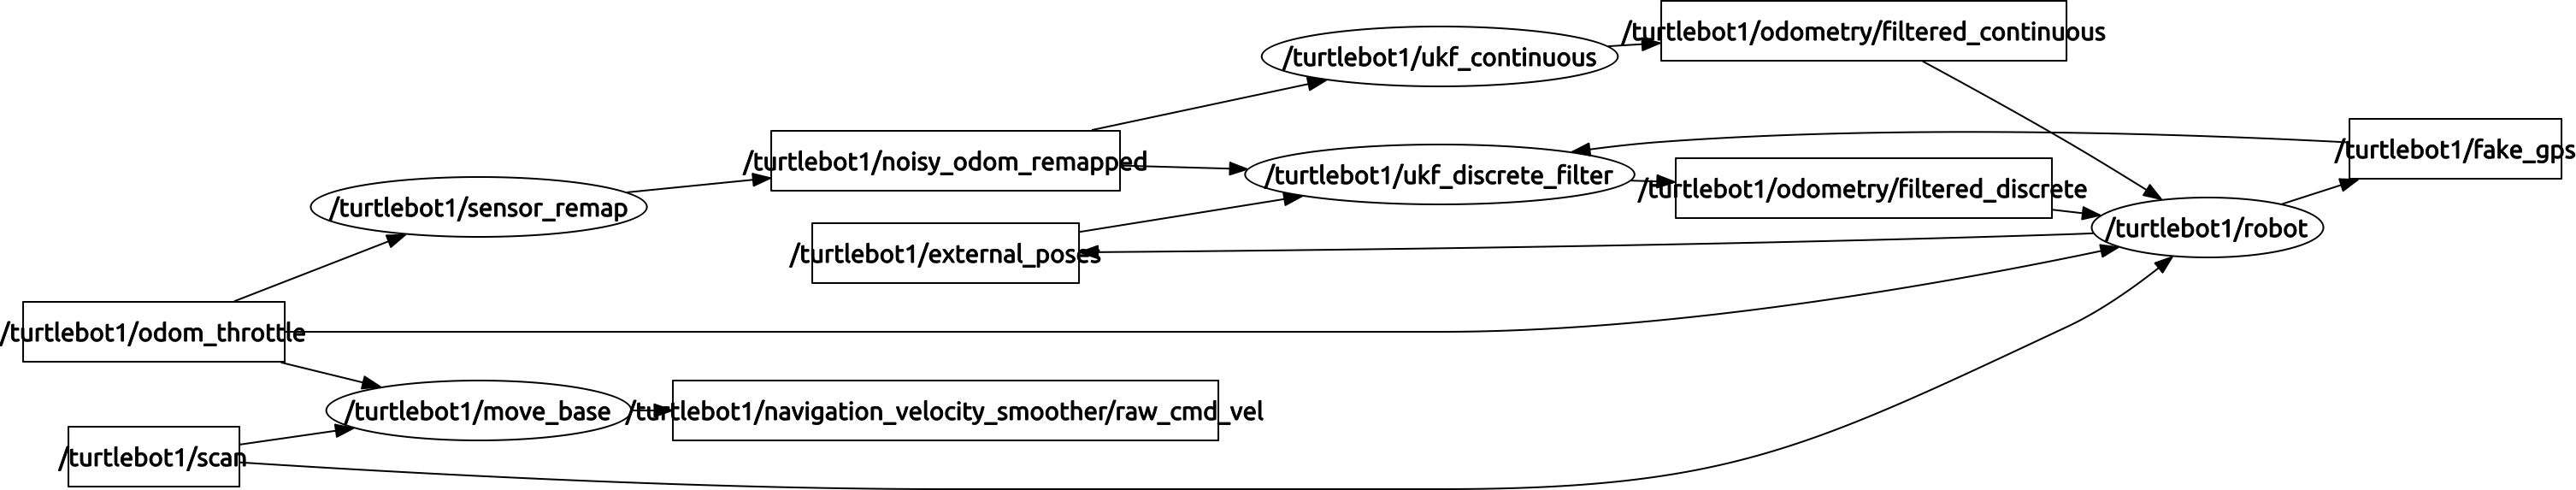
\includegraphics[width=\paperwidth, keepaspectratio]{simple_rosgraph}
\caption{ROS Node Structure}
\label{fig:node_graph}
\end{figure}
\end{landscape}

\subsubsection{Robot Node}
The robot node is where most of the heavy lifting is done for the robot. This node listens to the scan, which is a Lidar scan, and odom topics and calculates the external poses that are sent to other robots. It also sends movement commands to the move\_base node, but this is done via an action server and not a topic so it is not shown in this graph. The robot node also publishes the simulated GPS (fake\_gps) based on the robot's odometry information that is sent to the \gls{dist_filter}.

\subsubsection{Sensor Remap Node}
The sensor\_remap node subscribes to the odom topic, which is produced by the Gazebo simulator, and adds noise. The noise model is described in \autoref{sec:noise_model}.

\subsubsection{Filter Nodes}
The \gls{dist_filter} and \gls{con_filter} are both subscribed to the odometry information, adn the \gls{dist_filter} is additionally subscribed to the external poses and GPS.

\subsubsection{Move\_Base Node}
The move\_base node is the \gls{ros} navigation
\subsubsection{Unvisualized Nodes}
There are some unvisualized nodes.
\subsection{Communications Logic}
\subsection{Gazebo Simulation Details}
\subsection{Noise Model} \label{sec:noise_model}
\end{document}